\chapter{Sensor design}
This chapter will cover sensor basics, sensing element selection and theory of operation. The design will be presented at a system-level view. For a more detailed description of the electronics, please skip to chapter \ref{Engineering_model_chapter}.

\section{Review of commercially available RadFETs}
    Commercial solutions are based on a modified MOS structure (with thicker gate region). Example silicon structure is shown in figure \ref{Tyndall_radfet_silicon}. Different companies produce their own RadFET devices, by designing individual structures fitted to particular requirements. Researched companies only produce the RadFET sensors, leaving the readout circuit design for the customer to realise. A physical schematic and description for RadFET sensors is found in section \ref{Radiation_effects_on_MOS_transistors}. In table \ref{commercial_radfet_comparison} commercially available RadFETs are compared.

    \begin{figure}[H]
        \centering
        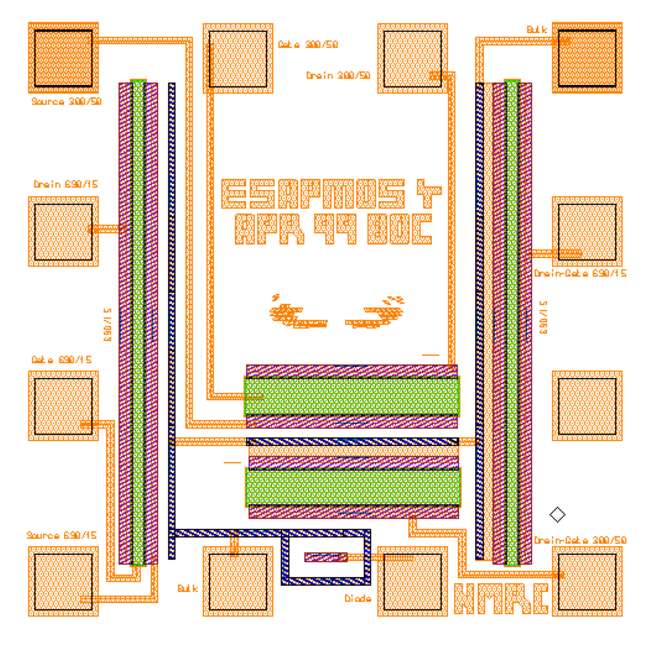
\includegraphics[width=0.5\paperwidth]{img/05/radfet-silicon.eps}
        \caption{4x RadFET silicon structure by Tyndall. Source: \cite{Tyndall_Radfet}}
        \label{Tyndall_radfet_silicon}
    \end{figure}

    \begin{table}[H]
    \begin{tabular}{| L{3.5cm} | C{3.5cm} | C{3.5cm} | C{3.5cm} |}
        \hline
        Type: & REM RFT300 & Tyndall TY1003 & Tyndall TY1004 \\ \hline

        Image: &
        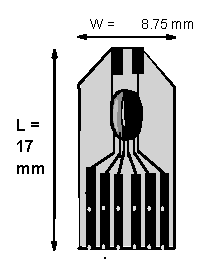
\includegraphics[width=0.15\paperwidth]{img/05/rem.eps} &
        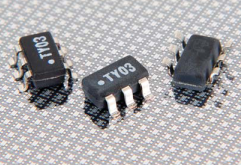
\includegraphics[width=0.15\paperwidth]{img/05/TY1003.png} &
        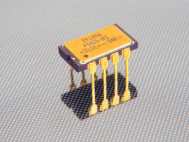
\includegraphics[width=0.15\paperwidth]{img/05/TY1004.png} \\ \hline

        Package: & custom & SOT23-6 & 8-pin ceramic DIL \\ \hline

        \# of transistors: & 2 & 2 & 2 \\  \hline

        Recommended readout current: & $10$ - \SI{500}{\micro\ampere} & \multicolumn{2}{c|}{\SI{10}{\micro\ampere}} \\ \hline

        TID dependency: & $n = 1$, $A~=~0.117$~\si{\milli\volt/\rad} & $n = 0.46$, $A~=~29.5$~\si{\milli\volt/\rad} & $n = 0.41$, $A~=~65.6$~\si{\milli\volt/\rad} \\ \hline
        Temperature readout: & diode & diode & diode \\ \hline
    \end{tabular}
    \caption{Commercial RadFET comparison}
    \label{commercial_radfet_comparison}
    \end{table}


\section{COTS MOSFET as RadFET}
    RadFETs are specifically designed MOSFETs that act as radiation sensors. However, the parameters of COTS MOSFET transistors also depend on total absorbed dose. They are much cheaper, but require proper calibration and testing in order to be considered as a flight solution.

    Many articles and papers prove that COTS MOSFETs can be used reliably as TID sensors. A number of available transistors were tested, their basic characteristics are compared in table \ref{cots_mosfet_comparison}. Parameters are taken at unbiased gate.

    \begin{table}[H]
    \begin{tabular}{| L{2cm} | C{2.4cm} | C{2.4cm} | C{2.4cm} | C{2.4cm} | C{2.4cm} |}
        \hline
        Type: & 3N163 & ZVP3306 & ZVP4525 & BS250F & CD4007 \\ \hline
        Reference: & \cite{3N163_article} & \cite{COTSMosfetsGarcia} & \cite{COTSMosfetsGarcia} & \cite{COTSMosfetsGarcia} & \cite{COTSMosfetsGarcia} \\ \hline

        Package: & TO-72 & TO-92 & SOT-223 & SOT-23 & TSSOP-14 \\ \hline

        $I_{ZTC}$ [\si{\micro\ampere}]: & 225 & - & - & - & 145 \\ \hline

        Sensitivity [\si{\milli\volt/\gray}]: & $24.3\pm 1.8$ & $3.7\pm 0.3$ & $3.4\pm 0.4$ & $3.1\pm 0.4$ & $4.6\pm 0.1$ \\ \hline

        $V_{TH_0} [\si{\volt}]$: & $2.0 - 3.0$ & $2.0 - 3.0$ & $1.5 - 2.5$ & $2.5 - 3.5$ & $1.9 - 2.5$ \\ \hline

        $V_{TH}$ @ \SI{100}{\gray} [\si{\volt}]: & $5.61$ & $3.4$ & $2.88$ & $3.85$ & $2.97$ \\ \hline
    \end{tabular}
    \caption{COTS MOSFET comparison}
    \label{cots_mosfet_comparison}
    \end{table}

    3N163 type have the greatest sensitivity - but bearing in mind the \SI{5}{\volt} supply for the sensor, it was discarded for too small range. The second best type is CD4007, which was selected for testing. Its parameters are suitable for the use under discussion, as shown in table \ref{CD4007_parameters}.

    Other advantages of CD4007 are:
    \begin{itemize}
        \item 3 P-MOS in one package - averaging/redundancy,
        \item additional diodes and transistors in device - possible temperature measurement
        \item small, vibration and thermally resistant package
    \end{itemize}

\section{Selected MOSFET - CD4007}
    The CD4007 consists of three complementary pairs of N- and P-channel enhancement mode MOS transistors. Internal connection diagram is shown below in figure \ref{CD4007_internal_diagram}. Predicted parameters of those transistors are collected in table \ref{CD4007_parameters}.

    \begin{figure}[H]
        \centering
        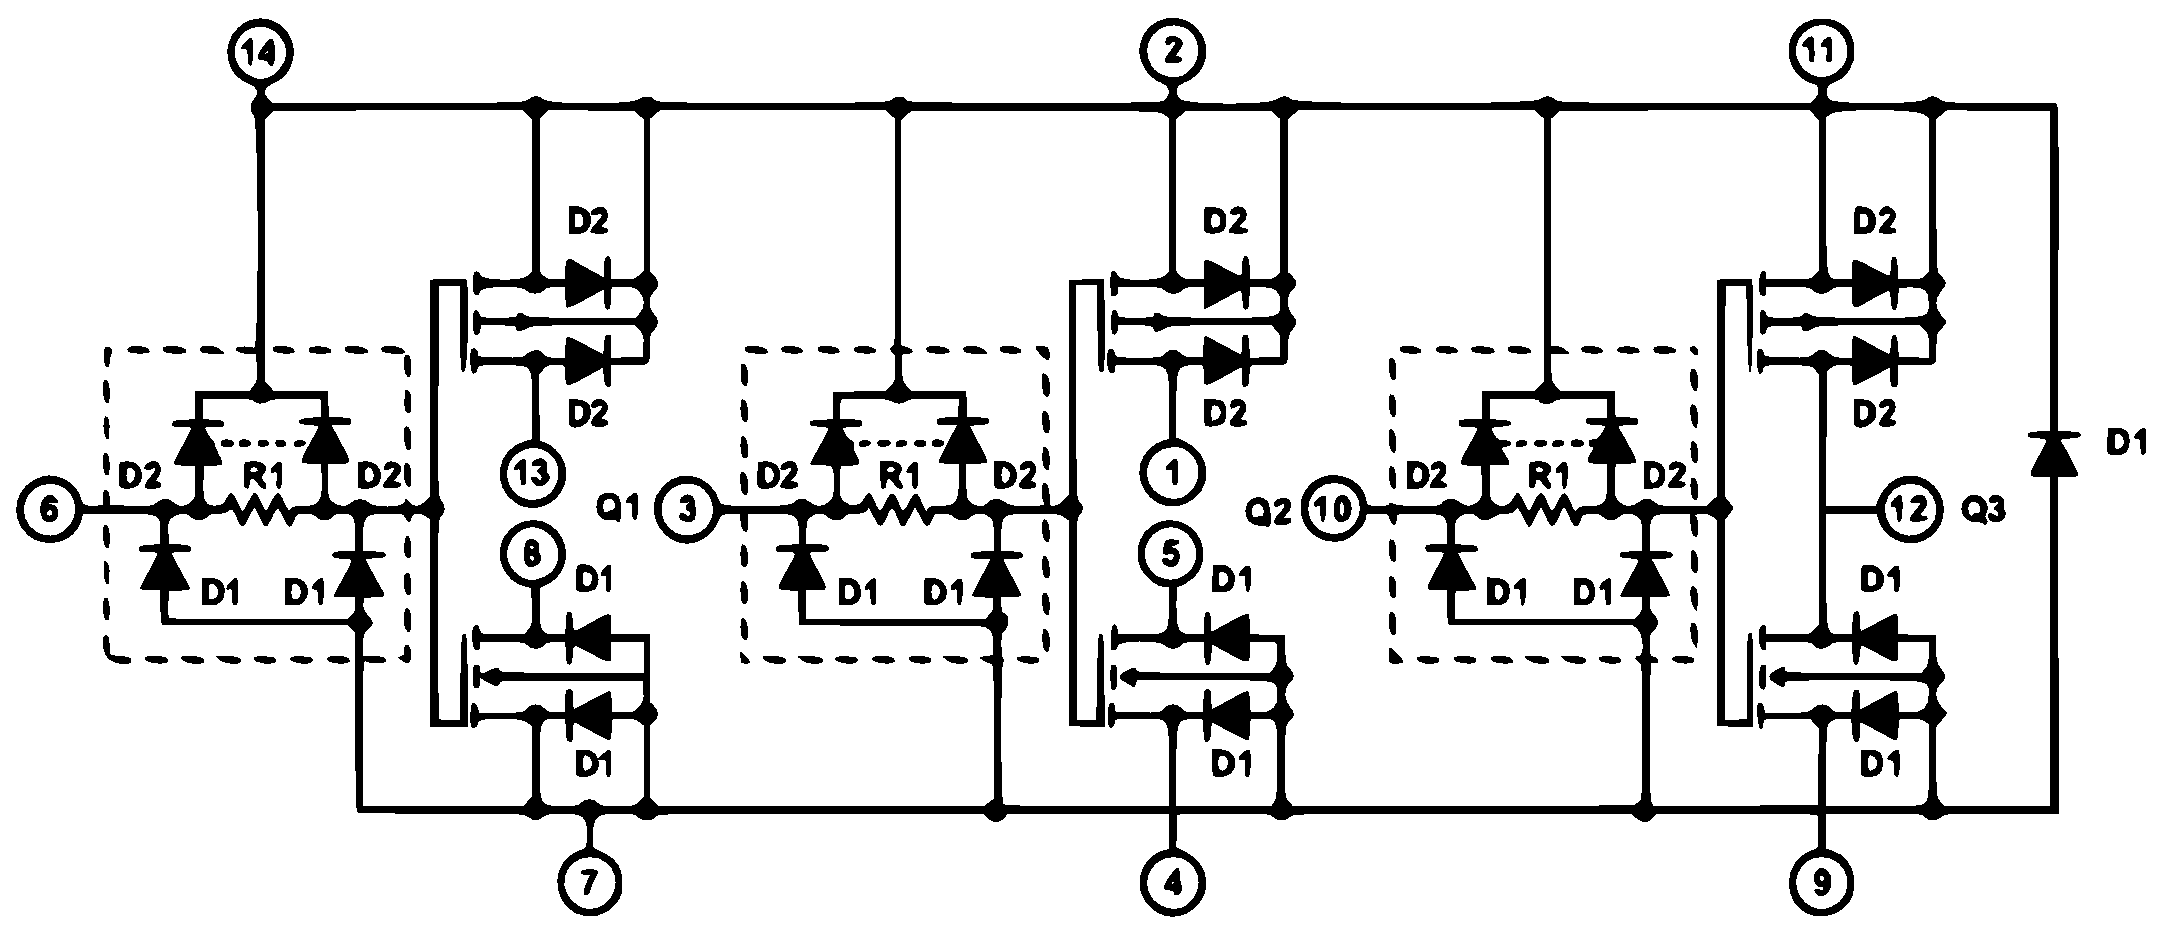
\includegraphics[width=0.7\paperwidth]{img/05/cd4007.eps}
        \caption{CD4007 internal diagram. Source: \cite{CD4007_schematic_functional}}
        \label{CD4007_internal_diagram}
    \end{figure}

    \begin{table}[H]
    \begin{tabular}{R{7cm} | L{7cm} }
        Transistor type: & 3x P-MOS and 3x N-MOS \\ \hline
        Supply voltage: & 3-18~\si{\volt} \\ \hline
        Threshold voltage: & \SI{1.8}{\volt} @ \SI{100}{\micro\ampere} \\ \hline
        Temperature range: & \SI{-55}{\degreeCelsius} - \SI{125}{\degreeCelsius} \\ \hline
        Zero-temperature coefficient current: & \SI{140}{\micro\ampere} \\ \hline
        Predicted sensitivity: & \SI{4.6}{\milli\volt/\gray}
    \end{tabular}
    \caption{CD4007 parameters}
    \label{CD4007_parameters}
    \end{table}

\section{Threshold voltage measurement}
    Threshold voltage changes with TID accumulated. The easiest method to measure change of this parameter is to connect the MOSFET in diode configuration, forcing constant drain current. A block diagram of this method is shown in figure \ref{Vth_readout_block_diagram}.

    \begin{figure}[H]
        \centering
        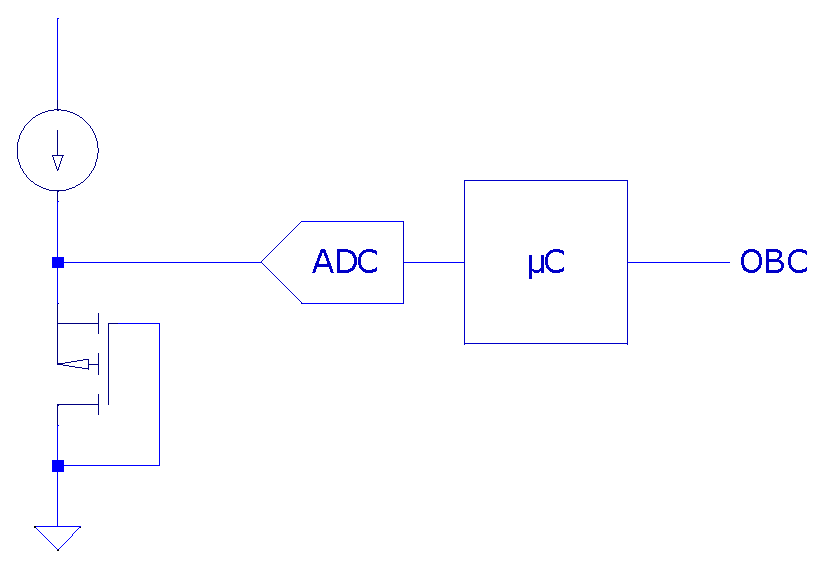
\includegraphics[width=0.3\paperwidth]{img/05/conceptual_block_diagram.eps}
        \caption{Threshold voltage readout block diagram}
        \label{Vth_readout_block_diagram}
    \end{figure}

    In saturation region, drain current is described by the following equation (body effect is negligible):

    $$I_D = A \cdot (V_{GS} - V_{th})^2$$
    Where:

    \begin{tabular}{lcl}
        $I_D$ & - & drain current \\
        $A = \frac{\mu_n C_{ox}}{2} \frac{W}{L}$ & - & constant for partuicular transistor \\
        $V_{GS}$ & - & gate-source voltage \\
        $V_{th}$ & - & threshold voltage \\
    \end{tabular}
    \bigskip

    Because only the threshold voltage change is of interest, measuring $V_{GS}$ has the same effect:
    $$I_D = A \cdot (V_{GS_1} - V_{th_1})^2 = A \cdot (V_{GS_2} - V_{th_2})^2$$
    $$\Delta V_{GS} = \Delta V_{th}$$

    The sensor should be shut down during irradiation - therefore no-bias method was used. It allows for complete isolation of supply power to the sensor, enabling it only for readout.

\section{Temperature measurement}
    Because threshold voltage strongly depends on die temperature, this effect has to be compensated for. The flight MOSFET will be calibrated in a thermal chamber prior to launch, thus obtaining characteristic curves.

    A number of possible temperature measurement techniques were considered during this thesis:
    \begin{table}[H]
    \begin{tabular}{R{4.5cm} | C{5cm} | C{5cm} }
        Method & Pros & Cons \\ \hline

        PT-1000 sensor glued to MOSFET & accurate reading & large thermal resistance, difficult assembly, low reliability \\ \hline

        ESD diode measurement in CD4007 & no additional sensor & complicated current, multiplexing circuit, unknown characteristics \\ \hline

        body diode in N-MOSFET in CD4007  & simple setup, reliable, known characteristics, low thermal resistance & no possibility of simultaneous readout of threshold and temperature (short thermal lag)
    \end{tabular}
    \caption{Temperature readout methods}
    \end{table}

    The chosen solution: to measure temperature of silicon die using body diode in complementary N-MOS transistor. A block diagram of this proposed solution is presented in figure \ref{Temperature_measurement_block_diagram}.

    \begin{figure}[H]
        \centering
        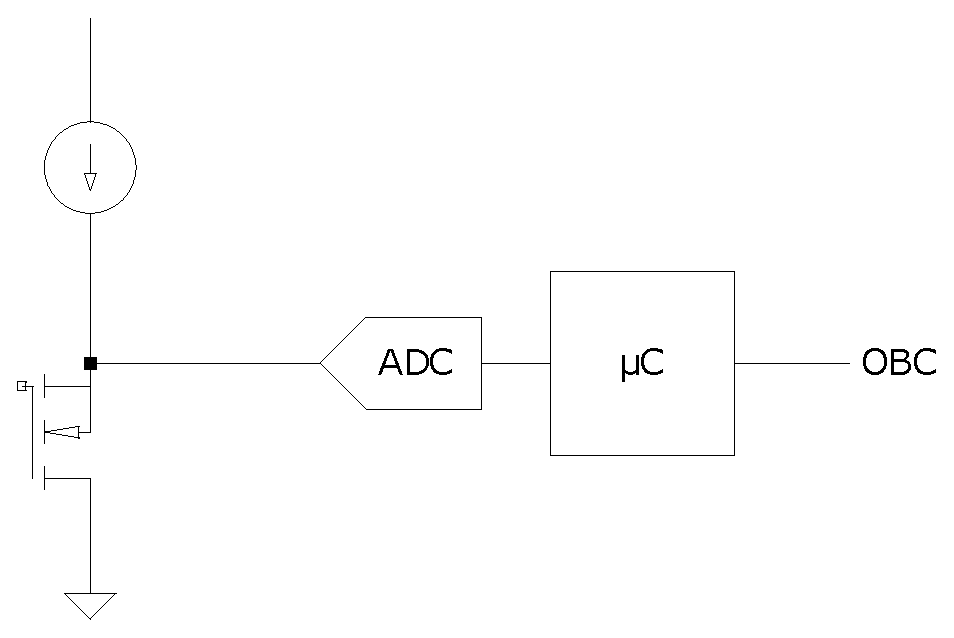
\includegraphics[width=0.3\paperwidth]{img/05/n-mos-temperature.eps}
        \caption{Temperature measurement block diagram}
        \label{Temperature_measurement_block_diagram}
    \end{figure}

    During calibration, both the temperature characteristics of the diode and the p-MOS threshold voltage will be obtained. They will be used to compensate for the threshold voltage shift associated with temperature. An individual flight component will be placed in a thermal chamber, and a proper look-up table will be created, with possible polynomial approximation.


\section{Characteristic curves}
\label{Characteristic_curves}

    During M. Gumiela's thesis, \cite{MGThesis} a calibration stand for CD4007 was developed. As an outcome of that project, rough calibration curves were obtained, which are presented below.

    \bigskip \textbf{p-MOSFET transfer characteristics}
    \begin{figure}[H]
        \centering
        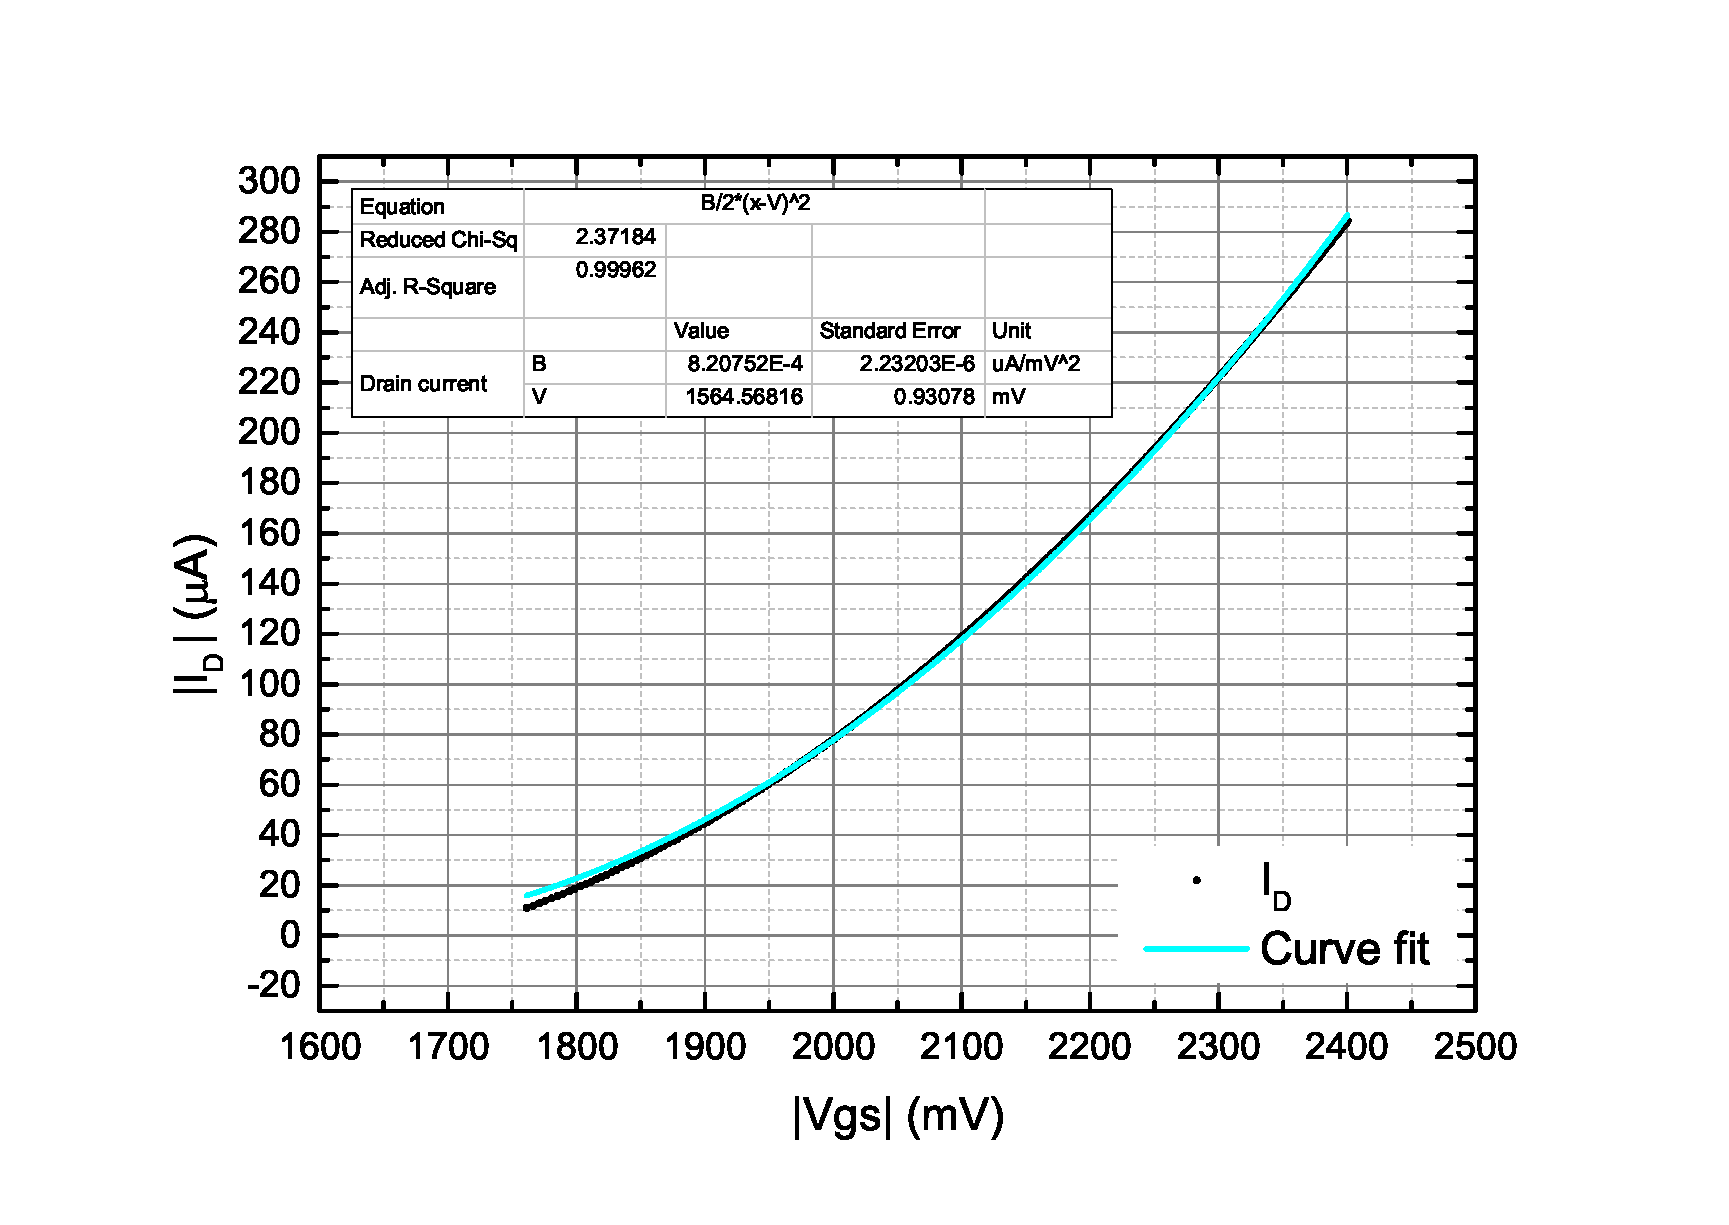
\includegraphics[width=0.7\paperwidth]{img/05/mg_iv_mosfet.eps}
        \caption{CD4007 p-MOSFET transfer characteristics. Source: \cite{MGThesis}}
        \label{CD4007_p-MOSFET_transfer}
    \end{figure}

    \bigskip \textbf{Linearized temperature coefficient of threshold voltage}
    \begin{figure}[H]
        \centering
        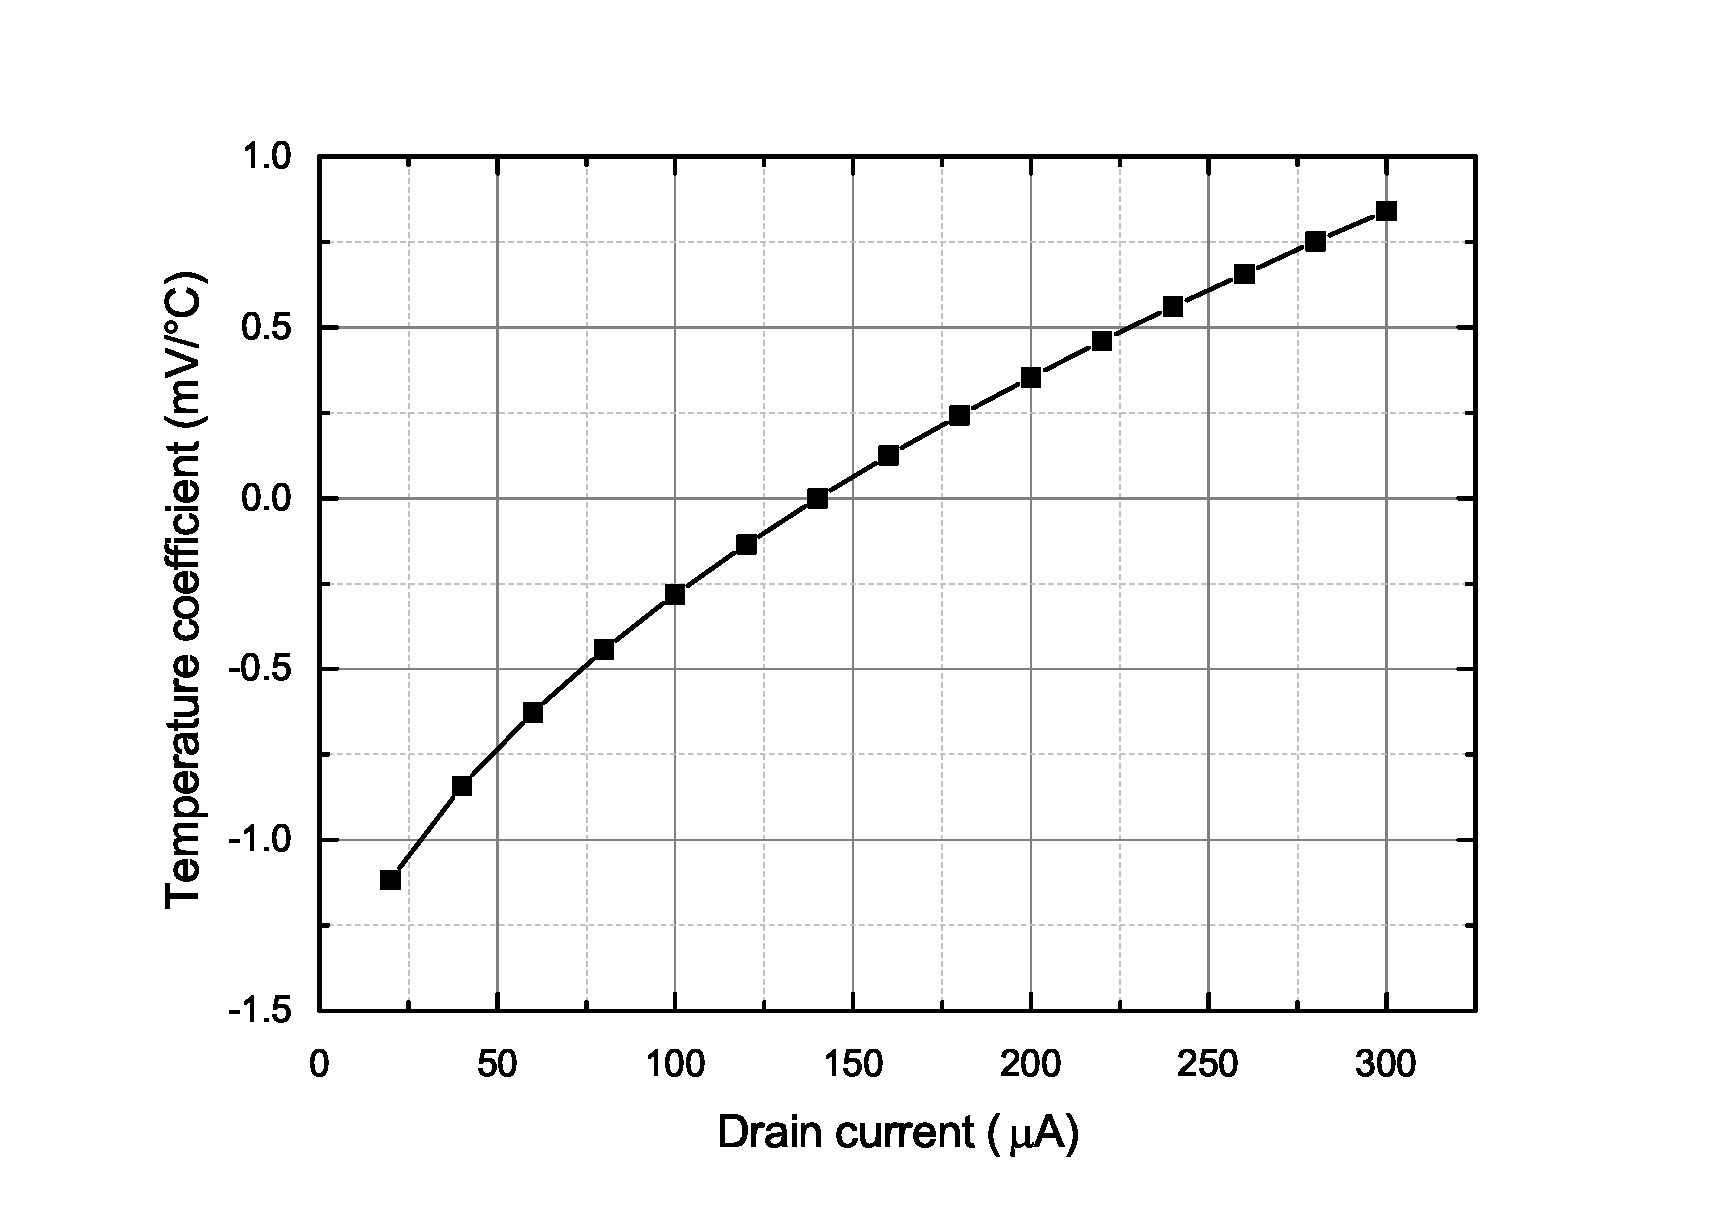
\includegraphics[width=0.7\paperwidth]{img/05/mg_tc_coefficients.eps}
        \caption{Linearized temperature coefficient of threshold voltage. Source: \cite{MGThesis}}
    \end{figure}

    \bigskip \textbf{Body diode forward voltage temperature calibration}
    \begin{figure}[H]
        \centering
        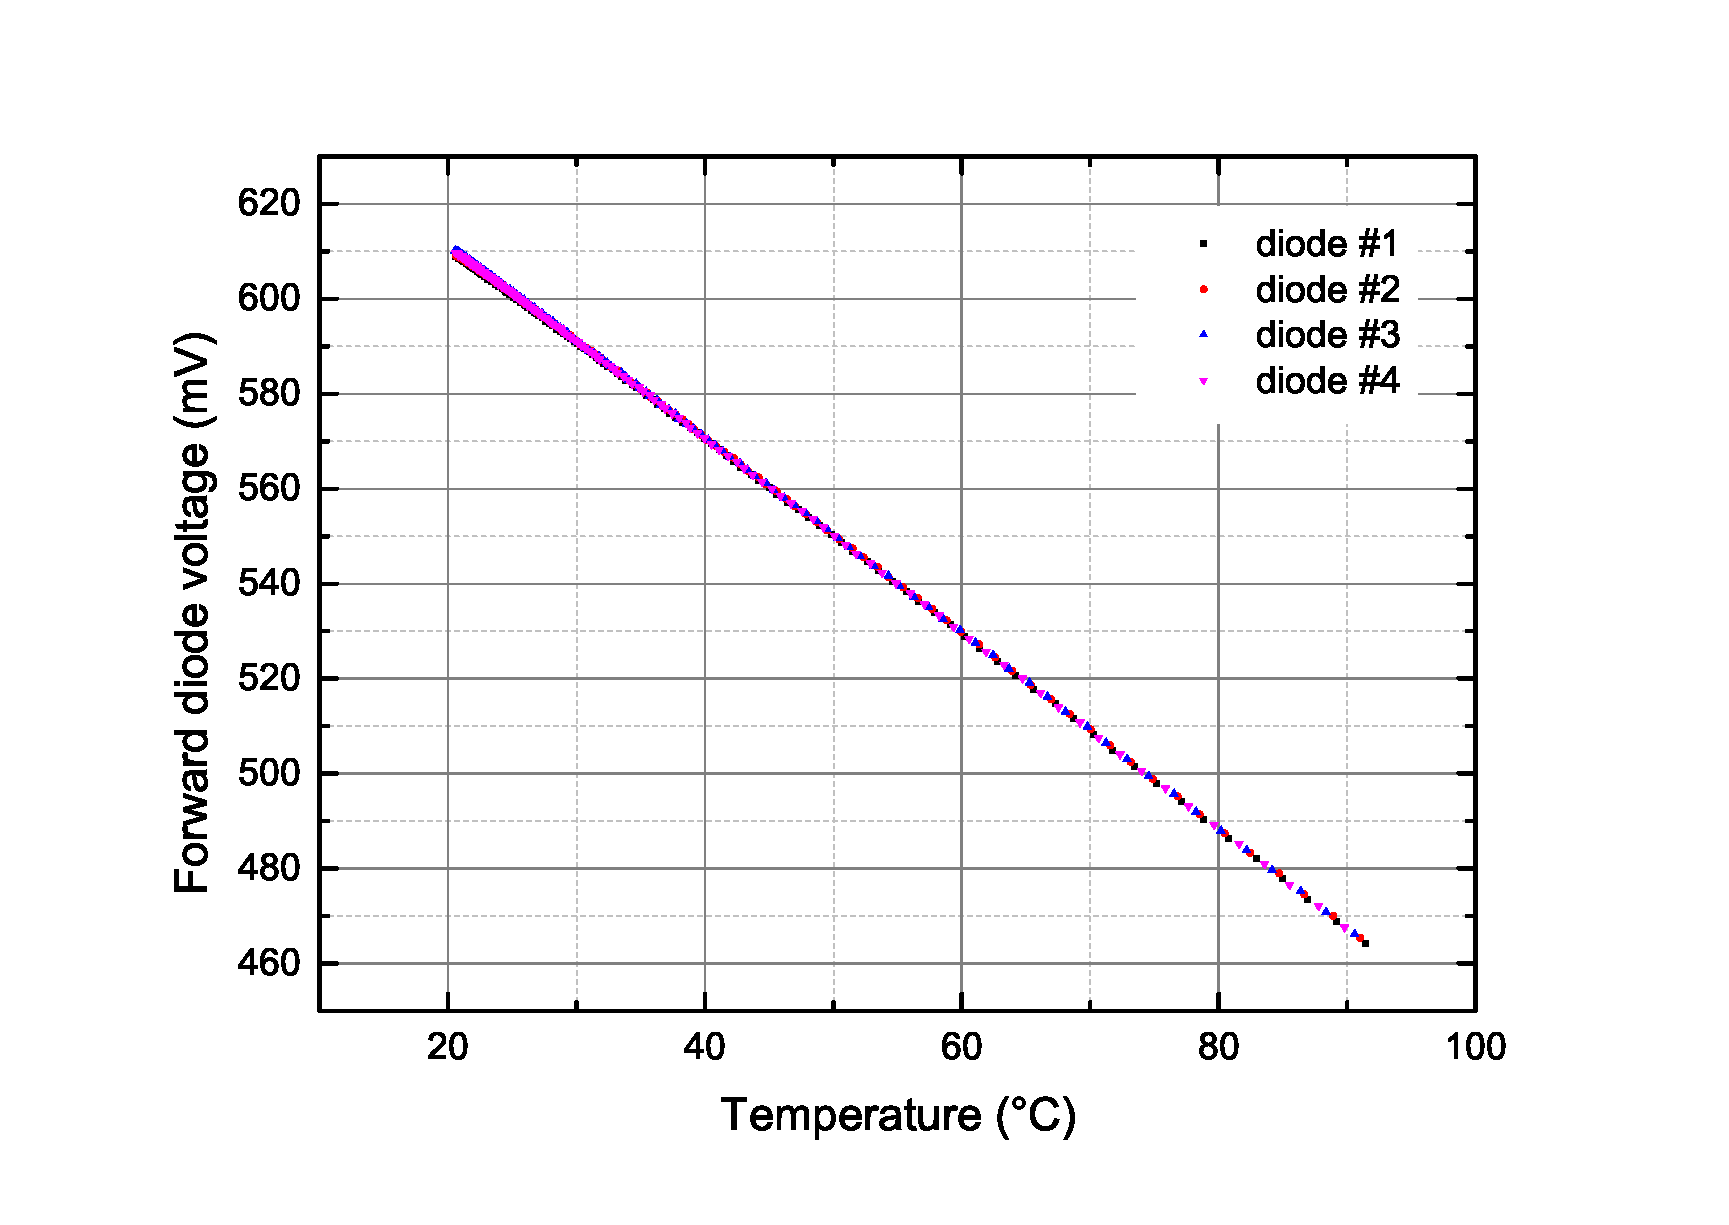
\includegraphics[width=0.7\paperwidth]{img/05/mg_diode_temp.eps}
        \caption{Body diode temperature calibration. Source: \cite{MGThesis}}
    \end{figure}

\section{Operating point selection}
    A current source value had to be chosen, keeping in mind the requirements and working conditions.

    In theory, a zero-temperature coefficient current would be optimal, but after irradiation it could shift slightly, causing a significant error. Additionally, due to limited availability of elements on the market and slight differences between devices, this operating point would be very difficult to achieve.

    As a tradeoff between low temperature coefficient and low starting threshold voltage, (to increase sensor range) the current value of \SI{125}{\micro\ampere} was chosen.
